\documentclass[11pt,a4paper]{article} 
\usepackage[danish]{babel}
\usepackage[utf8]{inputenc}
\usepackage{amsthm,amssymb,amsmath,dsfont,mathrsfs,nicefrac} 
\usepackage{graphicx}

\begin{document}

\section{Forside}

\section{Problemformulering}


\section{Indledning}


\section{Intruduktion}
Før jeg gik igang med dette projekt lagde jeg sjælden mærke til skyggeren i et rum. Selv om vi ikke ligger ret meget mærke til skygger ville verden se helt anderledes ud uden. Derfor er det også umuligt at lave en grafisk realistisk gengivelse af virkeligheden på en computer uden at på en eller anden måde at ligge skygger på.

\section{Hårde skygger}

I forbindelse med hårde skygge vil rapporten undersøge to forskellige måder at ligge hårde skygger på scenen, disse to forskellige måder arbejder enten i billede opløsning eller selve geometrien i scenen. Metoderne vil blive undersøgt, beskrevet, implementeret og tilsidste sammenlignet.

\begin{itemize}
  \item Shadow maps, arbejder i billedeopløsninger på scenen.
  \item Stencil shadow volumes, arbejder i selve geometrien på scenen.
\end{itemize}

\subsection{Forskellige shadow mapping metoder}

Dette afsnit vil undersøge nogle af de forskellige metoder at ligge skygge på en scene, der arbejder i billede opløsning. Tre af metoderne vil blive studeret og beskrevet. Fordele og ulemper opstilles og diskuteres, der vil herefter blive valgt en metode at gå i dybden med samt lave en implementering af denne. Metoderne som vil blive sammelignet er:

\begin{enumerate}
  \item Shadow mapping med Percentage Closer Filtering (PCF)
  \item Perspetive Shadow Mapping (PSM)
  \item Cascaded shadow maps (CSMs)
\end{enumerate}

Nr 1. er den "original" shadow mapping algoritme udgivet i 1987 \cite{SMAP}, rapporten vil dog kigge på algoritmen med Percentage Closer Filtering for løsning af aliasing problmer. Metode to og tre er modifikationen af nr. 1 disse modifikationen er lavet for at løse nogle af aliasing problemerne med shadow mapping algoritmen (Nr.1). De efterfølgende underafsnit vil kort forklare metoderne og herefter diskutere disse med henblik på at arbejde videre med den mest brug bare løsning.

\subsubsection{Shadow maps med PCF}

Shadow mapping \cite{SMAP} er en teknik der arbejder i billedopløsninger, ideen er at flytte kameratet op til lystkilden og tage et billede hvor kun dybderne gemmens(shadow mappet). Kameraet flyttes nu tilbage til øjet og for hver fragtment sammenlignes fragtmentes dybde med den sammen fragtment men projekteret over i shadow mappet, hvis dybden i shadow mappet er mindre er punktet i skygge fordi der er et punkt set fra kameraet der er nærmere. Da der kun arbejdes i billedopløsninger kan der opstå en del geometiske fejl samt over og undersamplings fejl der kan give fejlagtige skygger. Disse problemer kan tildels løses ved at bruge en bias og et filter kendt som Percentage Closer Filtering. Dette giver en tilfredsstillende algoritme.

Fordele
\begin{itemize}
  \item Hurtigt og egner sig godt til real-time grafik.
  \item Shadow mappet skal kun opdateres hvis lyset eller objekter flyttes ikke kameraet.
\end{itemize}

Ulemper:
\begin{itemize}
  \item Store aliasing problemer der dog tildels kan løses med PCF.
  \item Kræver scenen skal tegnes mindst to gange.
\end{itemize}


\subsubsection{Perspective Shadow maps}

Perspective Shadow Maps \cite{PSMAP} blev publiciteret i 2002 af Stamminger og Drettakis, denne metode bygger på videre på den originale shadow mapping ide \cite{SMAP}. Teknikken prøver at løse de alaising problemer der opstår i Shadow mapping, ved at justere den uniforme sampling fordeling i shadow mappet. Forbedring opnås ved at genere shadow mappet i \textit{Post-perspective Space} for kameraet, inden det perspective shadow map bliver generet bliver scenen og lyset transformeret med kamerates matrix. Dette betyder at objekter tæt på kameraet vil have en højere sampling, til forskel fra shadow mapping hvor samplingen factoren i forhold til objekter kun afhænger af deres placering i forhold til lyset og ikke kameraet.


Fordele
\begin{itemize}
  \item Løser i de fleste tilfælde aliasing problemer med shadow mapping
  \item Kræver ikke ekstra arbejde ved statiske scener og kamera.
\end{itemize}

Ulemper:
\begin{itemize}
  \item Shadow mappet skal generes  hver gang kameraet flyttes. Dette bevirker at algoritmen kræver en del mere arbejde en shadow mapping
  \item Objekter bagved kameraet der burde kaste skygge, kaster ikke skygge. Dette kan dog løses men giver andre problemer.
  \item Større problemer med Shadow acne.
  \item	Sensitive til the dueling frustum problemet (SKAL FORKLARES ET STED (VIST VED OVER/UNDER SAMPLING MEN NAVNET ER IKKE BRUGT) )
\end{itemize}

\subsubsection{Cascaded shadow maps}

Cascaded shadow maps har lidt af den samme ide som Perspective Shadow maps, nemlig at ligge præcisionen tæt på øjet og ikke lyset. Dog udvider Cascaded shadow maps denne tenik ved også at dele view fustrumet op så der optegnes flere shadow maps hvor præcisionen formindskes jo længere væk fra kameraet.  Dette bevirker at sampling kommer til at være mere ens med den der er behov for navnligt at der ligger meget præcision tæt på øjet hvor dette er nødvendigt og derved løser alaising problemerne.

\begin{figure}[ht!]
\centering
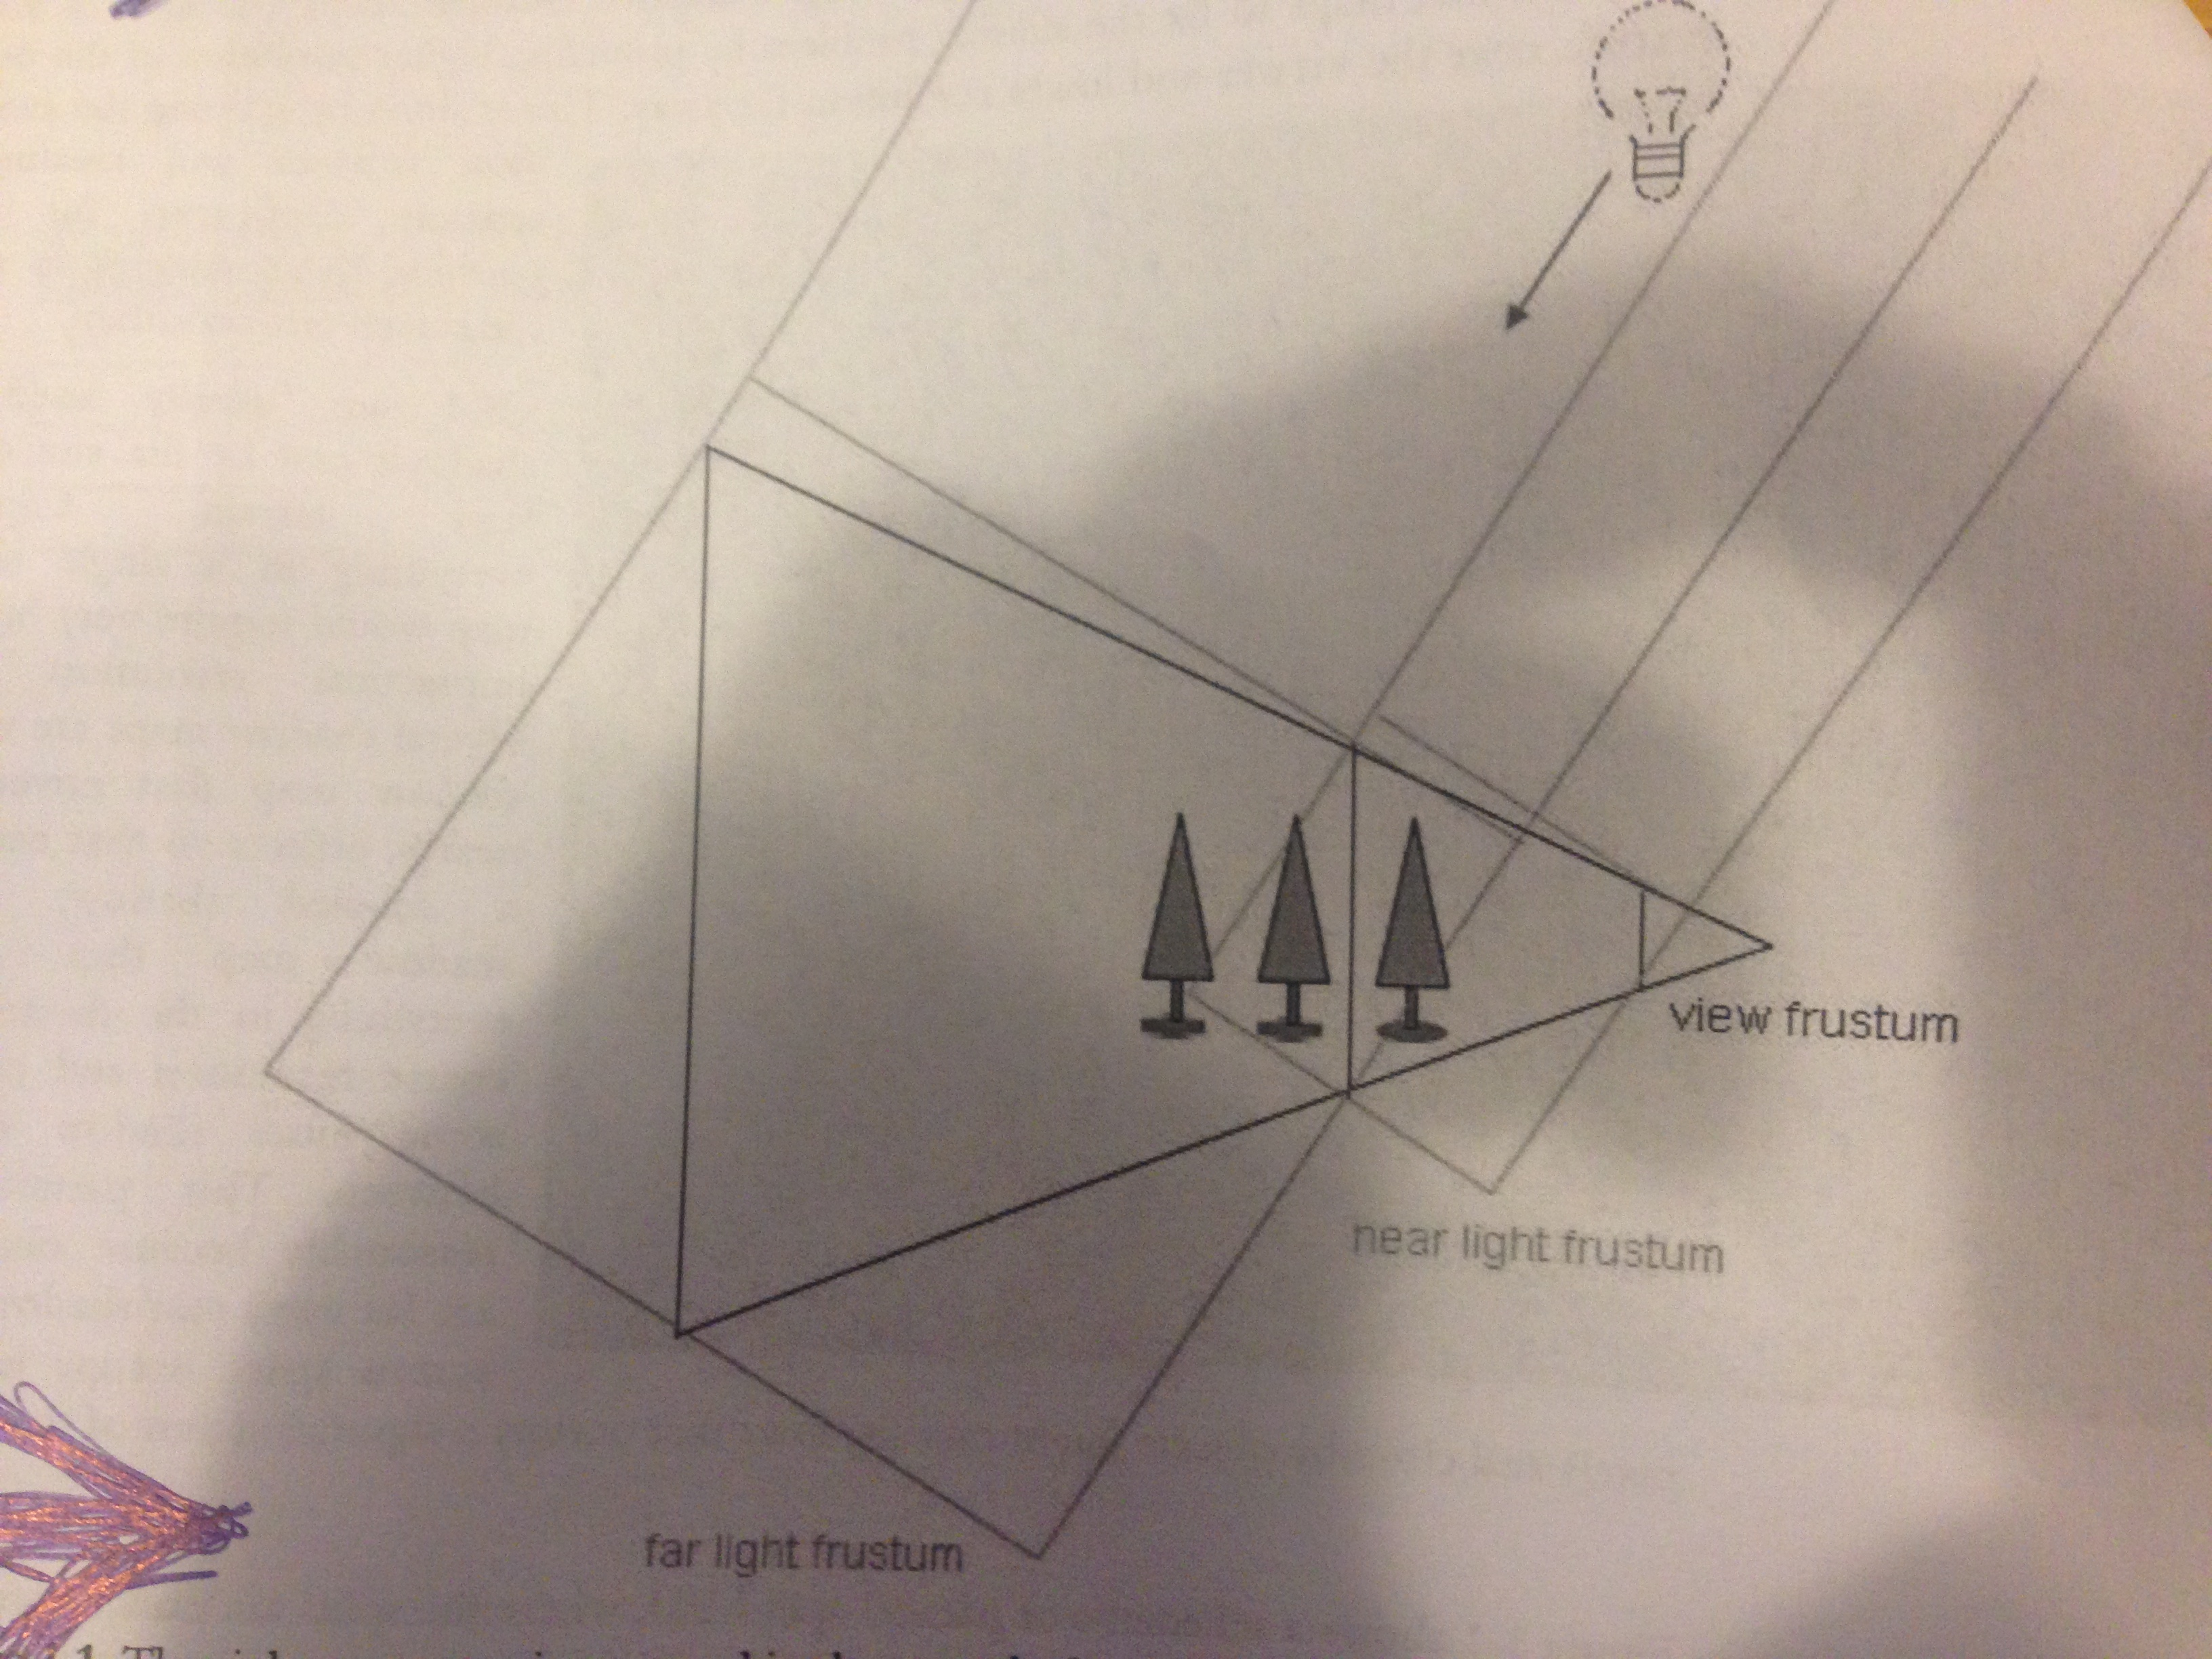
\includegraphics[width=140mm]{img/CSSHMAP1.JPG}
\caption{Shadow mapping teknikken}
\label{shadowmapdesc}
\end{figure}

Fordele
\begin{itemize}
  \item funger godt for store scenen hvor lyskilden er solen.
  \item Shadow mappet skal generes  hver gang kameraet flyttes. Dette bevirker at algoritmen kræver en del mere arbejde en shadow mapping
\end{itemize}

Ulemper:
\begin{itemize}
  \item Shadow mappet skal generes  hver gang kameraet flyttes. Dette bevirker at algoritmen kræver en del mere arbejde en shadow mapping
  \item
\end{itemize}

\subsubsection{Diskussion af shadow mapping algoritmer}


\newpage 
\section{Shadowmap}

Shadow maps blev indreduceret i 1987 af Lance Williams i artiklen "Casting curved shadows on curved surfaces". Siden er teknikken blevet brugt i film og computer grafik til at skyggelægge objekter.

Shadow mapping algoritmen arbejder kun i billedopløsninger og stiller derfor ingen særlige krav scenen anden end at den skal kunne tegens, dette gør at algoritmen hurtig samt meget fleksibel i forhold til valg af grafiske primitivere. Algoritmens styrke er dog også dens svaghed, dette skaber en del fejl skygninger og aliasing problemer som vil blive diskuteret i dette afsnit


\subsection{Teori}

En intuitive måde at finde ud af om et punkt er i skygge eller ej er forstille sig at man tegner en lige linje fra lyskildes origon til punktet A. Hvis denne linje rammer et eller flere punkter før den når punktet A, vil A være i  skygge ellers ikke. Figur \ref{shadowdesc} illustrere dette princip.

\begin{figure}[ht!]
\centering
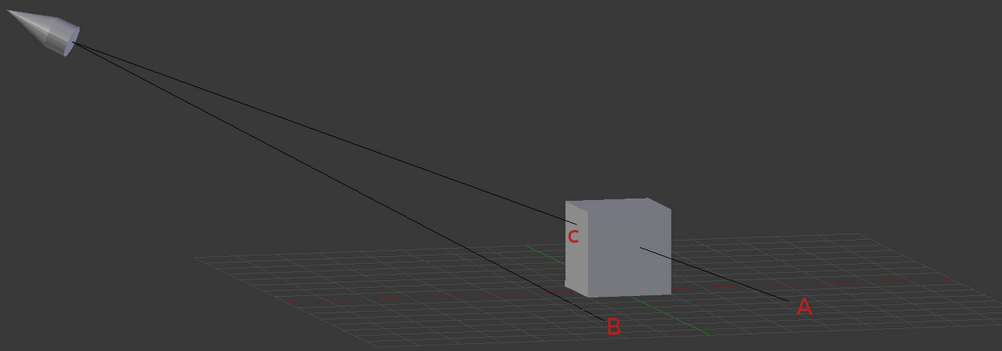
\includegraphics[width=120mm]{img/1.png}
\caption{Intuitiv forklaring af skygger. Punktet A ligger i skygge fordi den rette linie fra lyskilden til A går igennem C}
\label{shadowdesc}
\end{figure}

Det er netop denne tanke gang og en dybte buffer som shadow mapping udnytter. At skulle tegne linjer fra lyskilden til hvert punkt vil blive en meget kostelig affære, og det er her dybte bufferen bliver udnyttet. For når en 3D scenen projekteres til 2D billede, ses netop alle de alle punkter der er synlige fra kameraet, og hvis kameraet er i samme punkt som lyset vil disse også være de punkter der er synlige fra lyskilden. (Disse punkter og deres dybder gemmes i en dybde buffer beregnet til dette og kan senere bruges.)

Men dette i tankerne kan to steps algoritmen for shadow mapping nu beskrives således:
\begin{enumerate}
\item Scenen renderes set fra lyset men kun dybderne i scenen bliver gemt i dybde bufferen, det er denne der fungere som selve shadow mappet.
\item kameraet flyttes tilbage til øjet og scenen renderes. Hvert fragment projekteres over i lyset koordinatsystem og de to z-værdier sammenlignes. Er z-værdien i dybde buffere mindre er fragmentet i skygge.
\end{enumerate}

I step 1 er det kun dybder der er interessante og der kan derfor spares regne kraft på at udlade at rendere farver. Shadow mapping algorithem er visualiseret på figur \ref{shadowmapdesc}.


\begin{figure}[ht!]
\centering
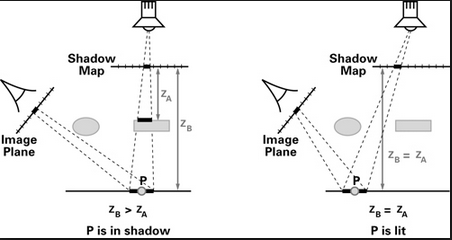
\includegraphics[width=140mm]{img/2.png}
\caption{Shadow mapping teknikken}
\label{shadowmapdesc}
\end{figure}


At kameraet bruges for at finde ud af hvad der er lyst op gør at denne metode egner sig godt ved brug af spotlight som lys kilde, dette kan dog udvides til andre lyskilder som fx. punkt lyskilder ved at tage billeder i alle retninger set fra lyste. Dette giver 6 shadow maps der sættes sammen i en kvadrat og derved få dybden for punkter set i alle retninger. Denne opgave vil kun arbejde med spotlight som lyskilder og i stedet fokusere på teknikker til at forbedre skyggerne der bliver kastet.  


\subsection{Praktisk}


Shadow mapping algoritmen er i teorien er meget simpel, men når algoritmen bruges praktisk kan der opstå mange fejl der gør at algoritmen ikke giver et godt resultat. Disse problemer opstår især fordi shadow mappet er en diskret repræsentation af scene 

Disse problemer er:
\begin{enumerate}
\item Front og back clipping plan.
\item Numerisk unøjagtighed ved dybte sammen ligning.
\item Geometrisk unøjagtighed ved projektion(opstår bla. pga. undersampling).
\item Oversampling (Opstår når et fragtment i kamera space mappes til mange punkter i shadow mappet)
\item Undersampling (Opstår når mange fragtment i kamera space mappes til et eller få punkter i shadow mappet)
\end{enumerate}

Det første problem med shadow mapping der skal tages hånd om er clipping planerne i visningstuben (view frustum). For at algoritmen skal fungere korret er det vigtigt at alle objekter er inden for back clipping planet når scenen optegnes fra lyse, ellers vil objekterne fejlagtigt kommer i skygge selv om lyskilden kaster lys uendeligt langt væk og der ikke er noget der blokere lyset. Dette skyldes at ved opslaget i shadow mappet for objekter der ligger udenfor back-clipping plantet vil denne dybde værdi altid være større end den for shadow mappet. Løsning på problem 1, er at sørge for at back-clipping planet bag det bagerste objekt i scene, dette virker dog kun for afgrænsede scener. En anden løsning er helt at undlade back-clipping planet(Dette skal jeg undersøgt betydningen af). Det samme problem opstår med front-clipping planet og også her er løsningen at dette opsættes så ingen objekter ligger melle dette og kameraet. Problem 5 er illustreret på figur \ref{P1}. 

\begin{figure}[ht!]
\centering
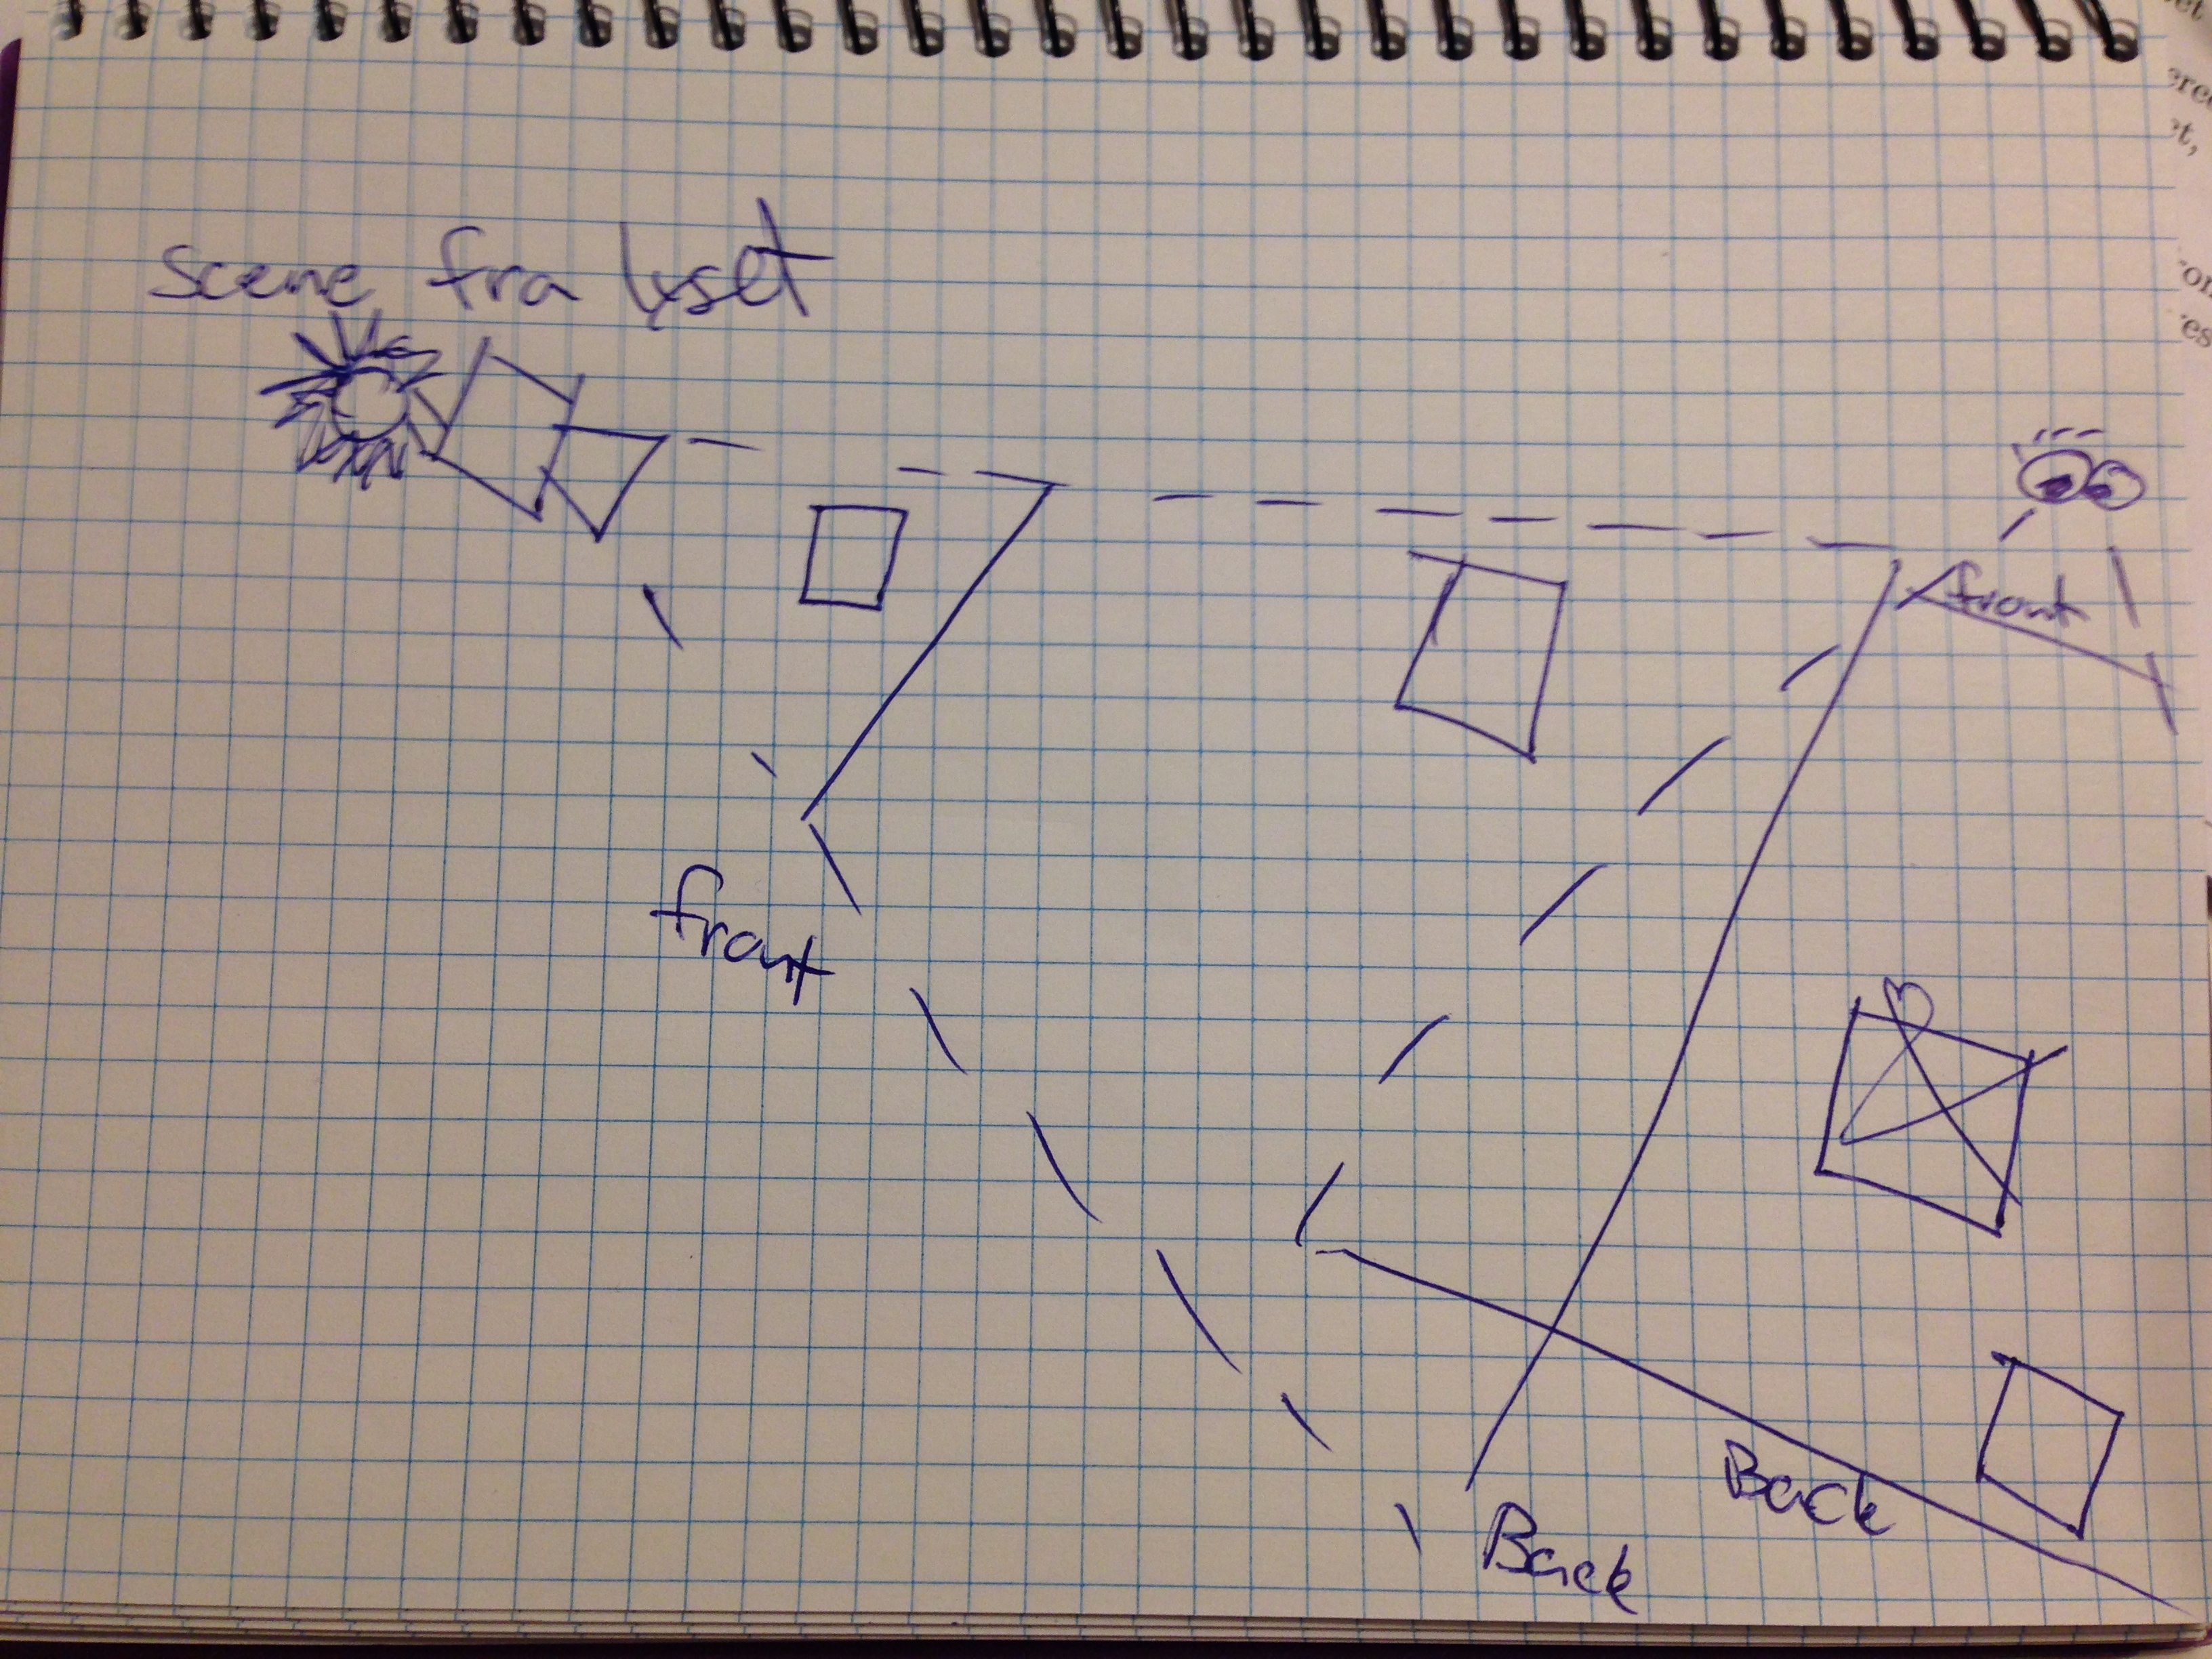
\includegraphics[width=90mm]{img/P1.jpg}
\caption{Problem med back-clipping planet ved optegning af shadow mappet.}
\label{P1}
\end{figure}

Problem 2 og 3 ses ved at objekter i scenen fejlagtigt kaster skygge på sig selv, fænomenet er også kendt som shadow acne og er beskrevet i afsnittet af samme navn i rapporten. Shadow acne kan løses ved at indføre en tolerance (bias) ved sammenligning af z-værdierne. Hvilket beskrives i Biasing afsnittet.

Oversampling opstår når et fragtment i kamera space mappes til mange punkter i shadow mappet, dette kan være et problem i realtids programmer da dette skaber unødvendigt meget arbejde, samtidig kan skygger også forekomme rystelser i skyggerne. Undersampling opstår når shadow mappet ikke indeholder tilstrækkelig information, dette er en fordel i realtids programmer, dog kan skygger forekomme meget kantede og nogle steder forkerte.  Dette opstår fordi der bliver brugt en perspektiv projektion, hvilket betyder at der er meget information tæt på front clipping planet og meget mindre ude ved back-clipping planet. Hvis kameraet er placeret i den anden enden af scenen vil dette give undersampling da mange pixel tæt på kameraet skal projekteres til meget få pixel i sahdow mappet. Problemet er illustreret i 2D på figur \ref{P2}.  Både over og under-samplings problemet vil blive forsøgt forbedret i Percentage Closer Filtering (PCF) afsnittet.


\begin{figure}[ht!]
\centering
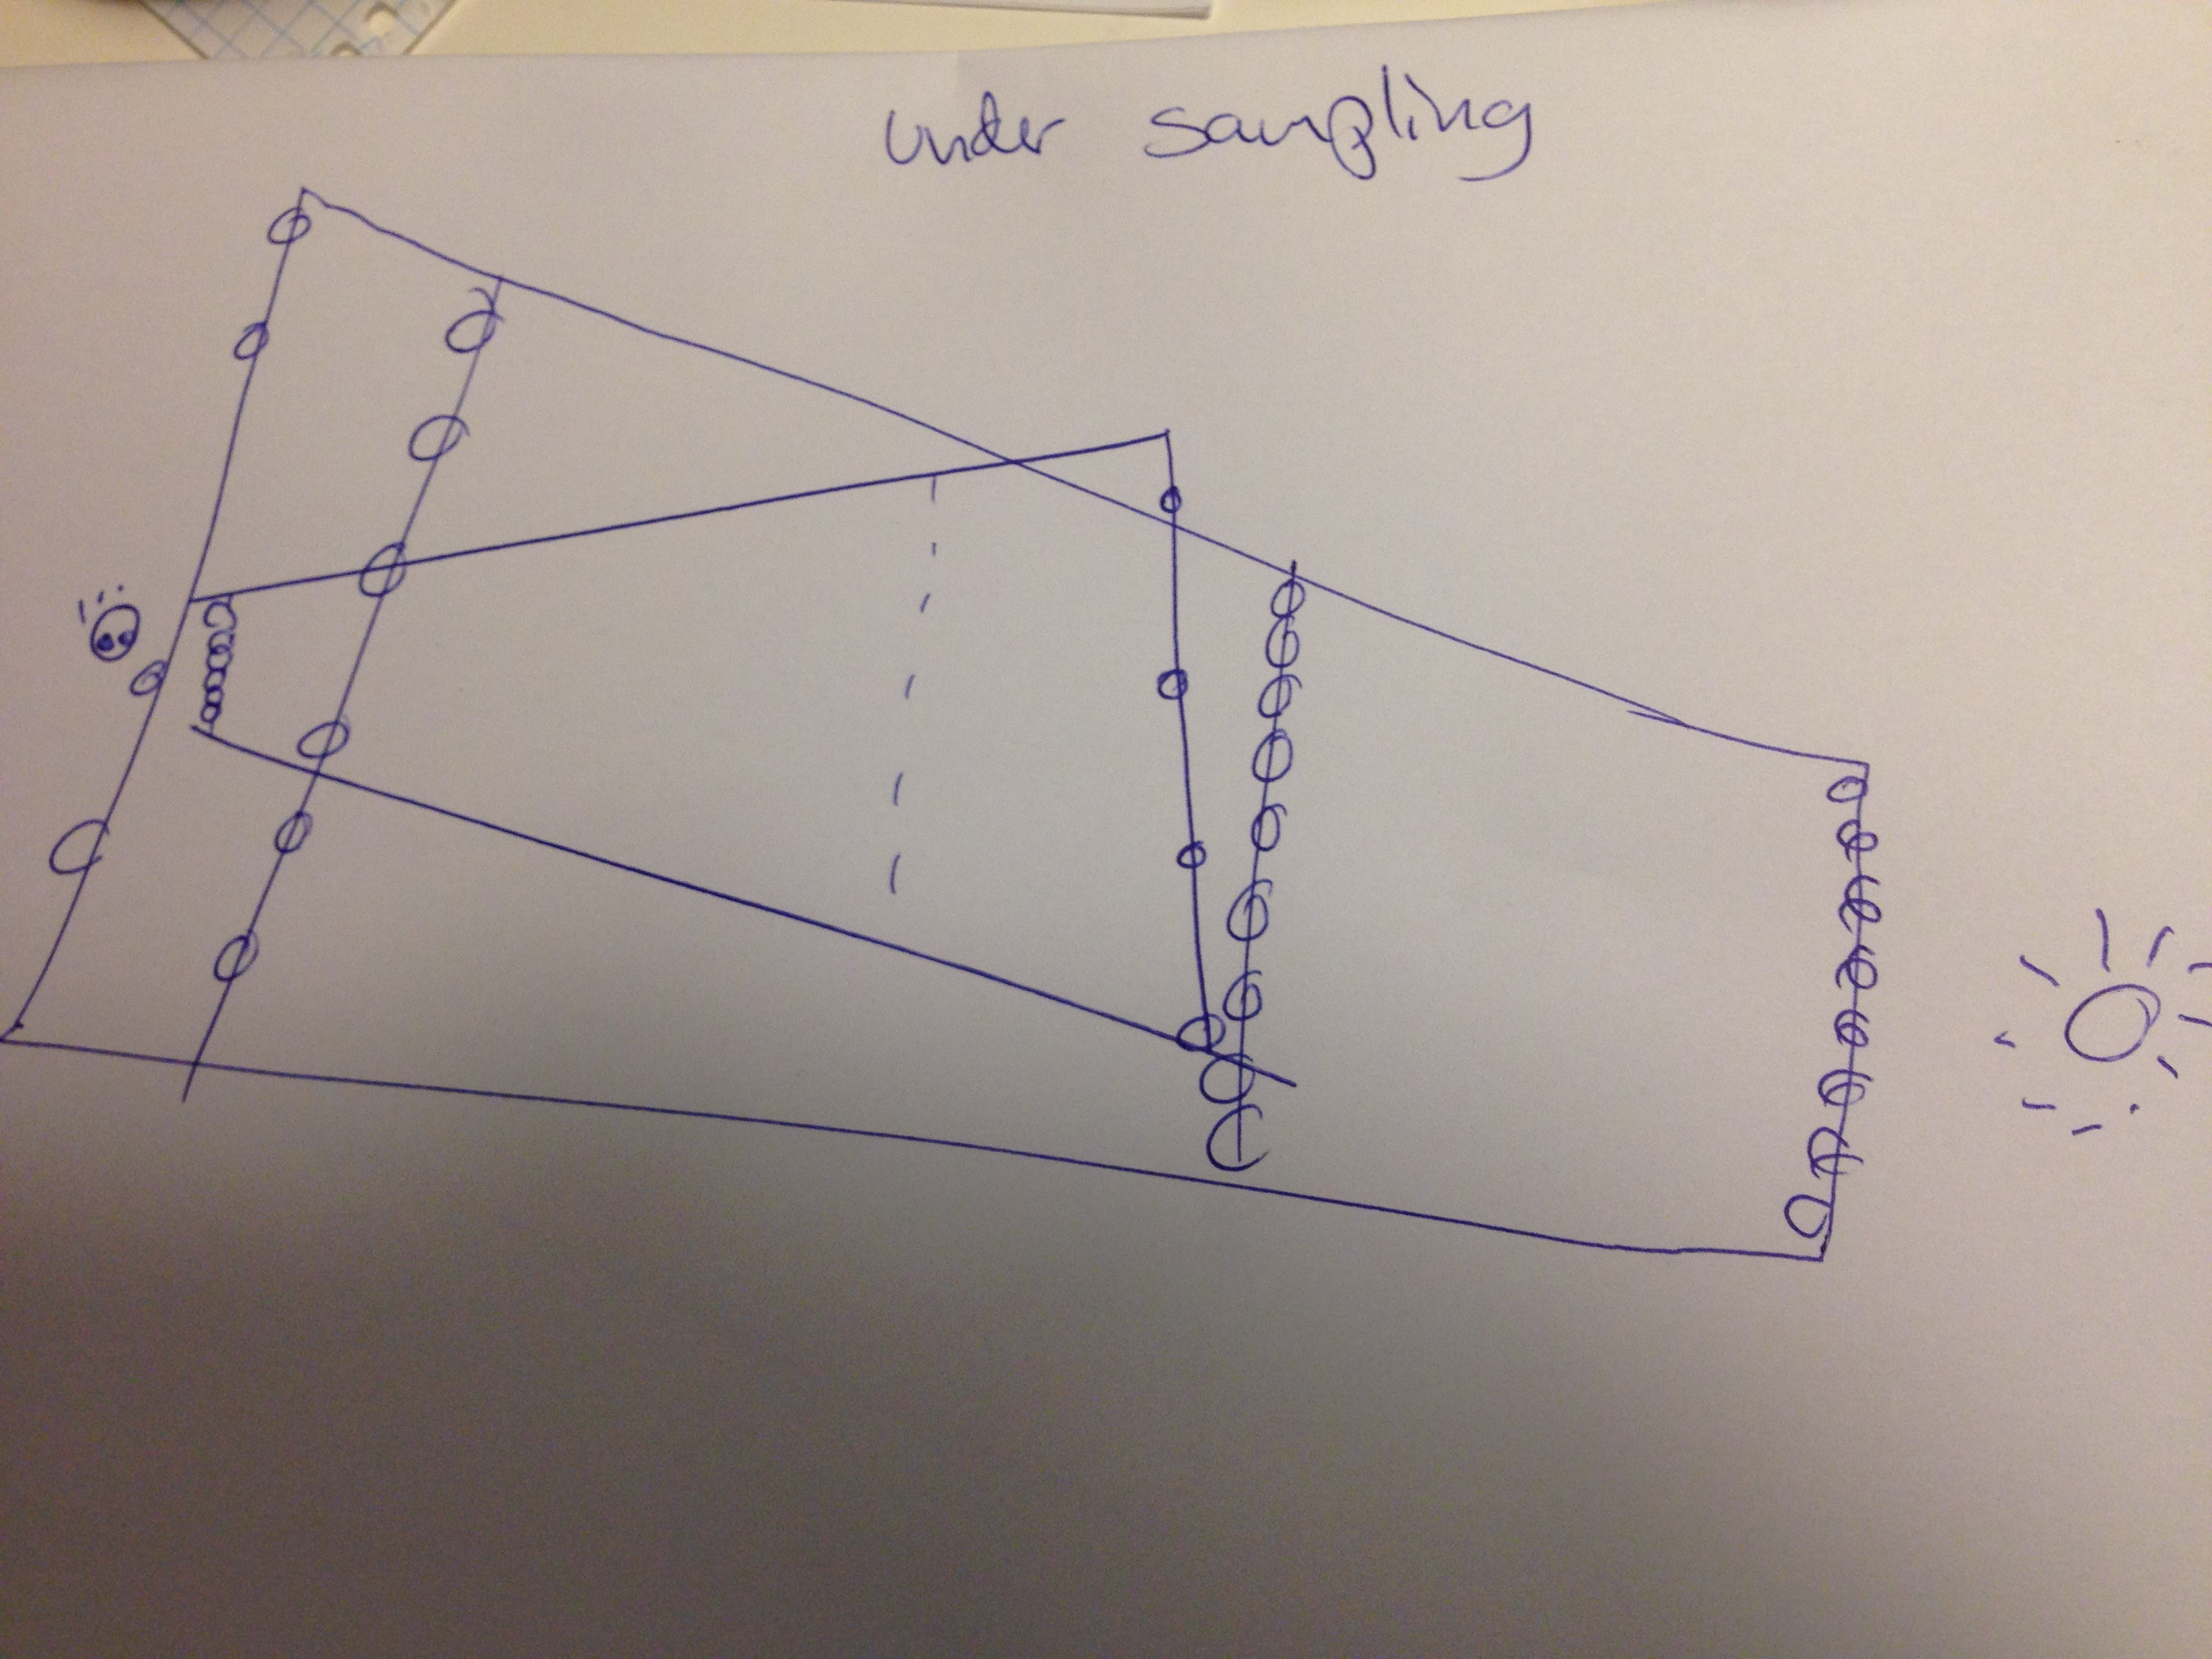
\includegraphics[width=90mm]{img/P2.jpg}
\caption{Undersampling. Et meget stort antal pixel fra kamerate skal mappes til kun 3 pixel i shadow mappet.}
\label{P2}
\end{figure}


\subsubsection{Shadow acne}

Det mest synlige problem med shadow mapping algritmen er \textit{self-shadowing alising} bedre kendt som \textit{shadow acne}, hvor et  polygon fejlagtigt kaster skygge på sig selv. Der er to grunde til at dette problem opstår, den første  er at decimaler smides væk fordi der dybde buffer indeholder flydende tal. Dybde buffer har et vis antal bit til at repræsentere det flydende tal for z-værdien,  og som altid når der regnes flyenden tal kan der opstår afrundings fejl. Denne afrundings fejl kan betyde at når de 2 z-værdier sammenlignes er disse ikke helt ens og polygonet kan derfor fejlagtigt kaste skygge på sig selv.  Se figur \ref{S0}.

\begin{figure}[ht!]
\centering
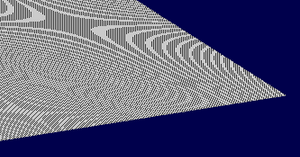
\includegraphics[width=90mm]{img/S0.png}
\caption{Shadow acne}
\label{S0}
\end{figure}

En af de ting der skyldes shadow acne at der ikke er præcision nok i dybde kortet, denne præcision kan forbedres ved at rykke  "front"  og "back" clipping planerne så de tætter indkapsler alle objekterne i scenen. Dette vil dog ikke kun fjerne shadow acne helt men forbedre resultat samt forbedre resultat når andre metoder tages i brug. 


Den anden grund til at \textit{shadow acne} opstår er geometriske fejl. Disse geometriske fejl forekommer fordi dybde værdien for et punkt sample bliver brugt til at beskrive dybden for et areal. Når et punkt fra kameraet projekteres ind i shadow mappet vil disse to punkt sample sjældent være helt det sammen og derfor vil dybde værdierne heller ikke være helt den sammen, dette problem er illustreret på figur \ref{S1}(a).

\begin{figure}[ht!]
\centering
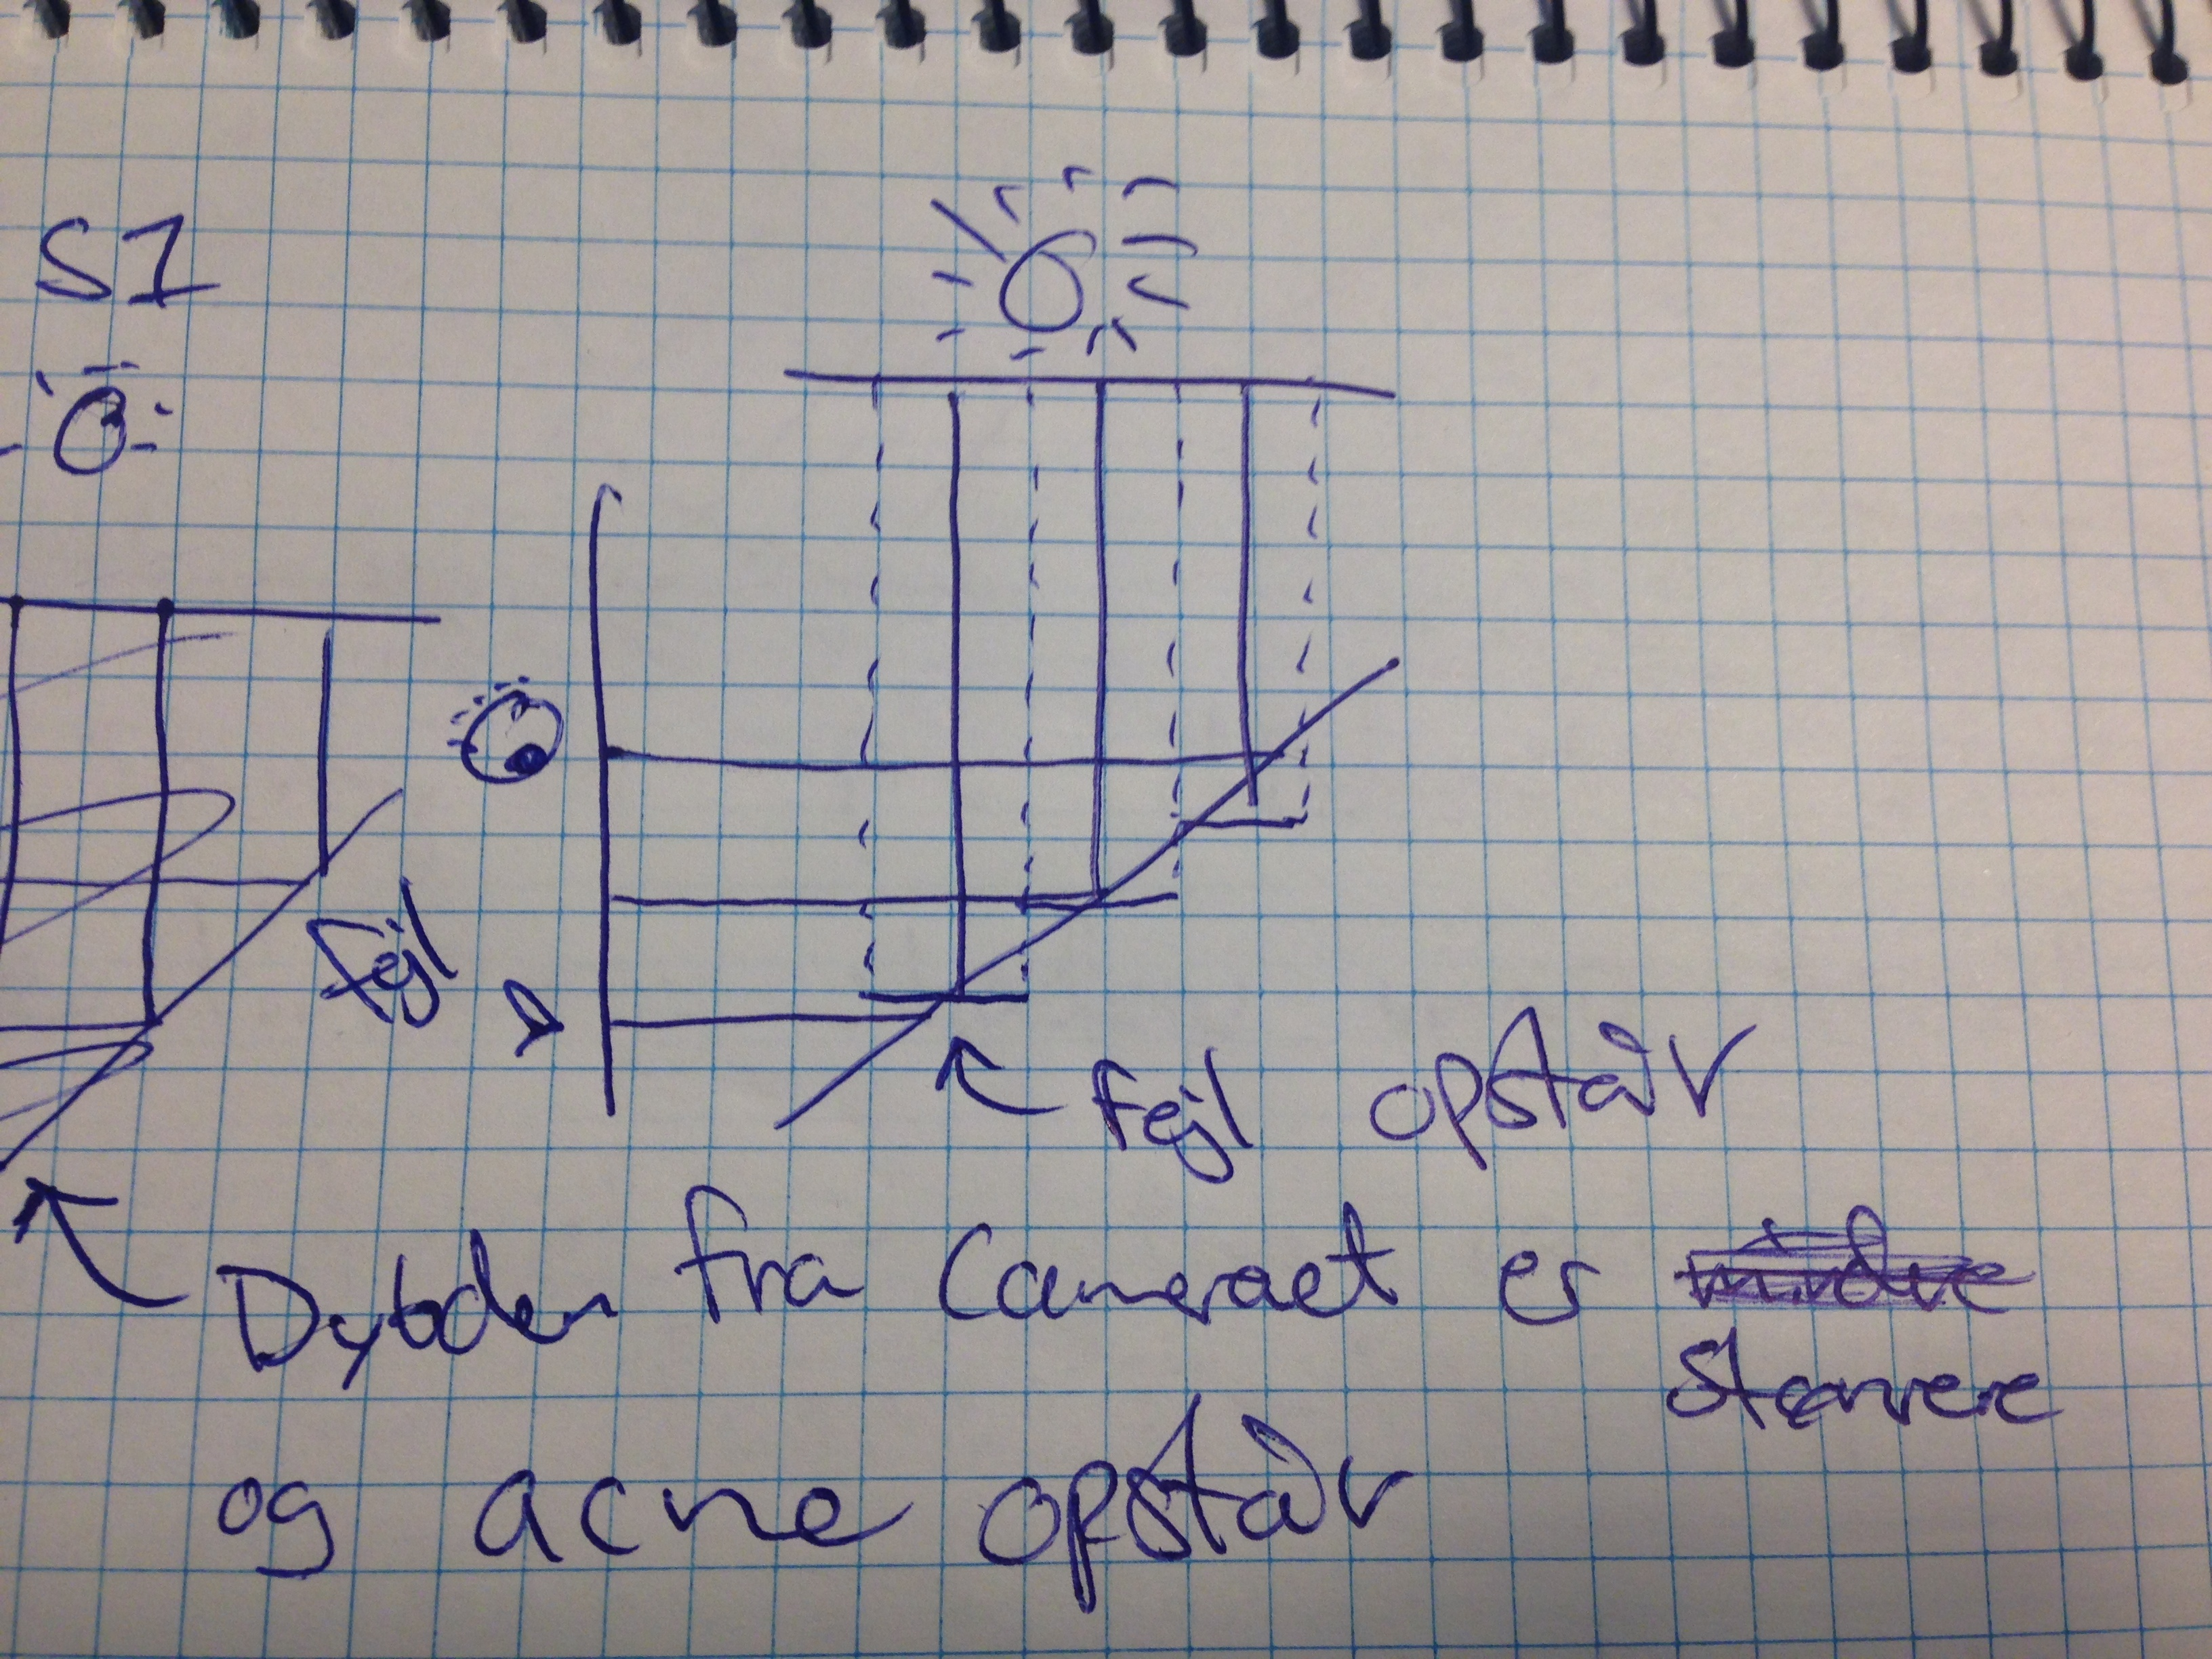
\includegraphics[width=90mm]{img/S1.jpg}
\caption{Shadow acne opstår fordi punkt samplet ikke er helt ens set fra lyset og øjet.}
\label{S1}
\end{figure}

Det ses på \ref{S1}(a) at hvis punkt samplet ikke er helt ens set fra lyset og øjet vil det nogle gange gå godt hvor z-væredien set fra øjet vil være mindre eller lig den set fra lyset mens det andre gang vil opstå selv skygning fordi z-værdien er større set fra øjet. \textit{shadow acne} er så stort problem at der skal tages hånd om det for at shadow mapping algoritmen kan give et acceptabelt resultat. Løsning på dette problem er at indføre en bias værdi der flytter alle polygoners z-værdi en lille smule når dybde kortet optegnes. Det næste afsnit vil forklare hvordan denne bias værdi vælges og anvendes.


\subsubsection{Biasing}

Biasing er en måde at håndtere shadow acne problemet på, biasing løser shadow acne problemet det at sørge for at dybde fra øjet(kameratet) = < dybde i shadowmappet for alle fragtmenter fra det samme polygonium.  Bias er et lille offset der adderes til z-værdien inden dybde testen i opengl foretages og derved bliver alle fragtmenter flyttet lidt tilbage og vil derfor ikke kunne skygge for sig selv se figur \ref{S2}(b). Dette vil i mange tilfælde løse shadow arne.

\begin{figure}[ht!]
\centering
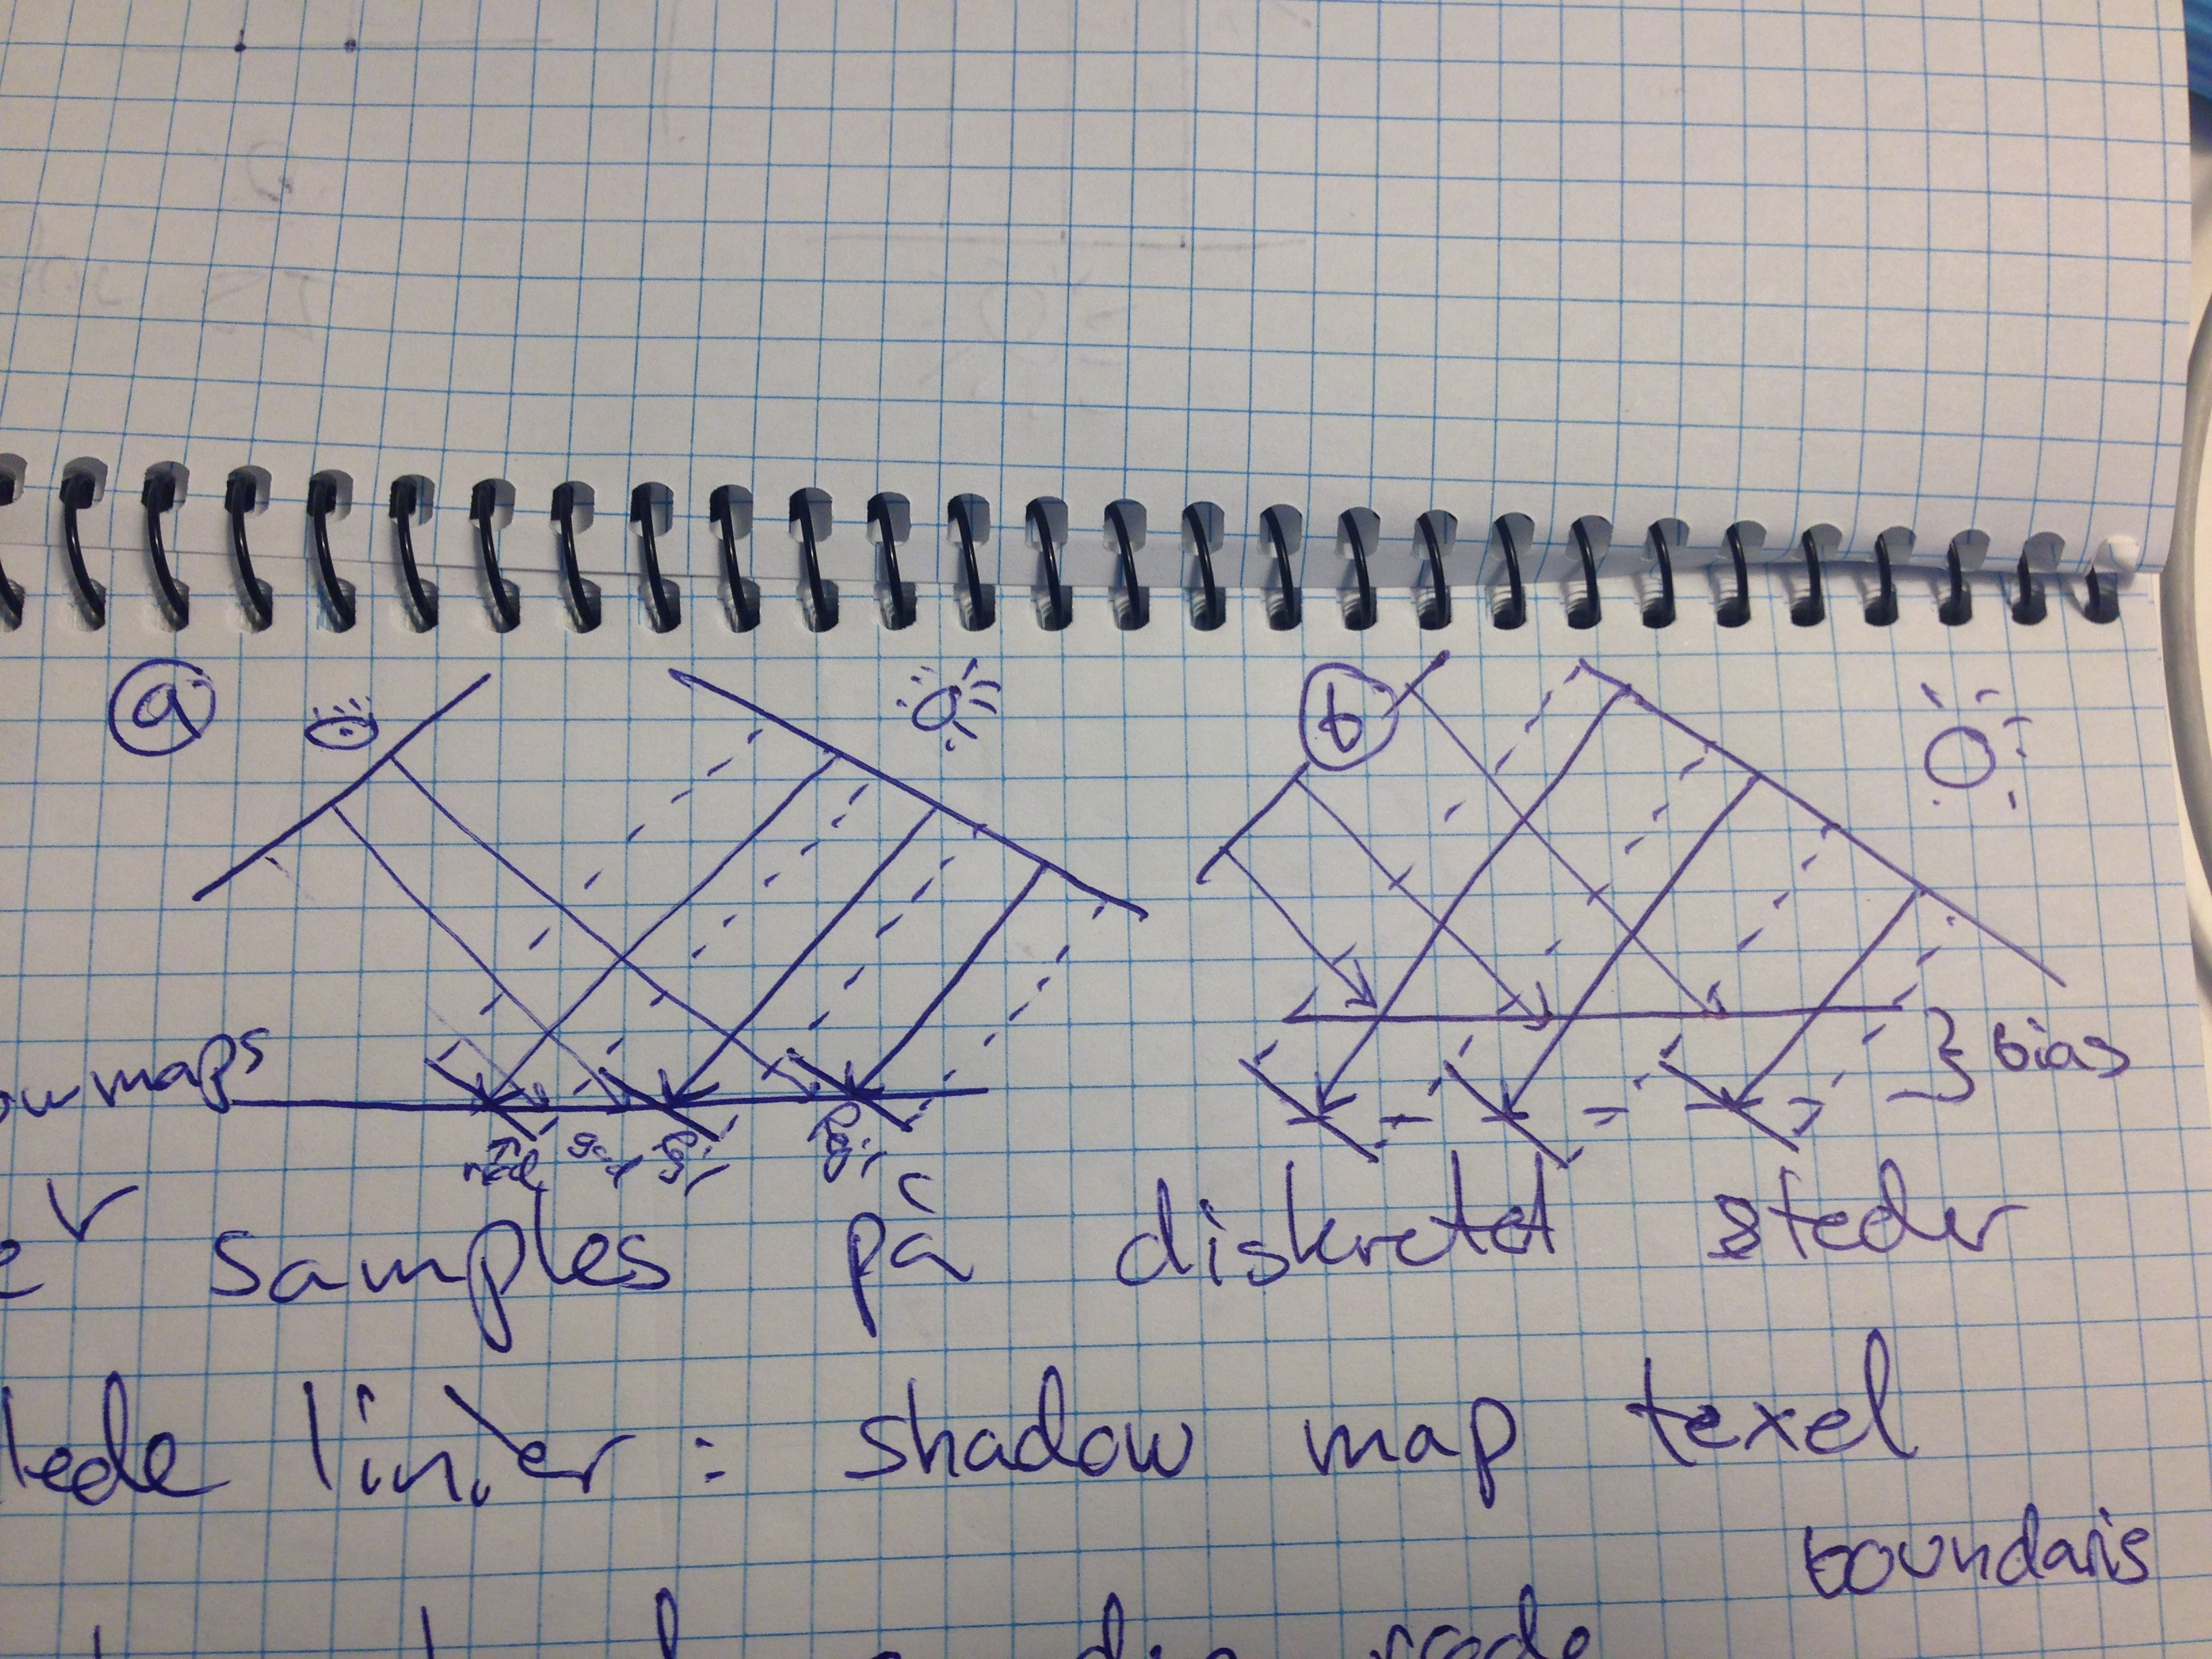
\includegraphics[width=80mm]{img/S2.jpg}
\caption{Pile er shadow map samples på diskrete steder. Stiplede linier er shadow map texel afgrænsninger.For hver texel er den røde linie den dybde shadow mappet gemmer. Figur (b) ses betydningen af biasen, dybde værdierne fra øjet vil nu altid være større for samme polygon og der opstår derfor ikke geometrisk eller numerisk fejl.}
\label{S2}
\end{figure}

I den simpleste form er biasing en konstant offset værdi der tilføjes til fragmentet, denne værdi er dog ikke så lige til at vælge fordi størrelsen af  værdi bliver nød til at ændre sige i forhold til vinklen mellem projektions planet for lyset og fladen på det polygonie der kastes lys på. Desto mere vinkelret de to planer er på hinanden jo større bias er der behov for. Som det ses på figur \ref{S3} er det ikke altid at en konstant bias værdi kan løse shadow acne problemet, hertil kan bruges en \textit{slop-scale bais} der har til formål at blive større i takt med vinklen mellem  projektions planet for lyset og fladen på det polygonie vokser, derved sørge for at bias værdien altid er stor nok. 


\begin{figure}[ht!]
\centering
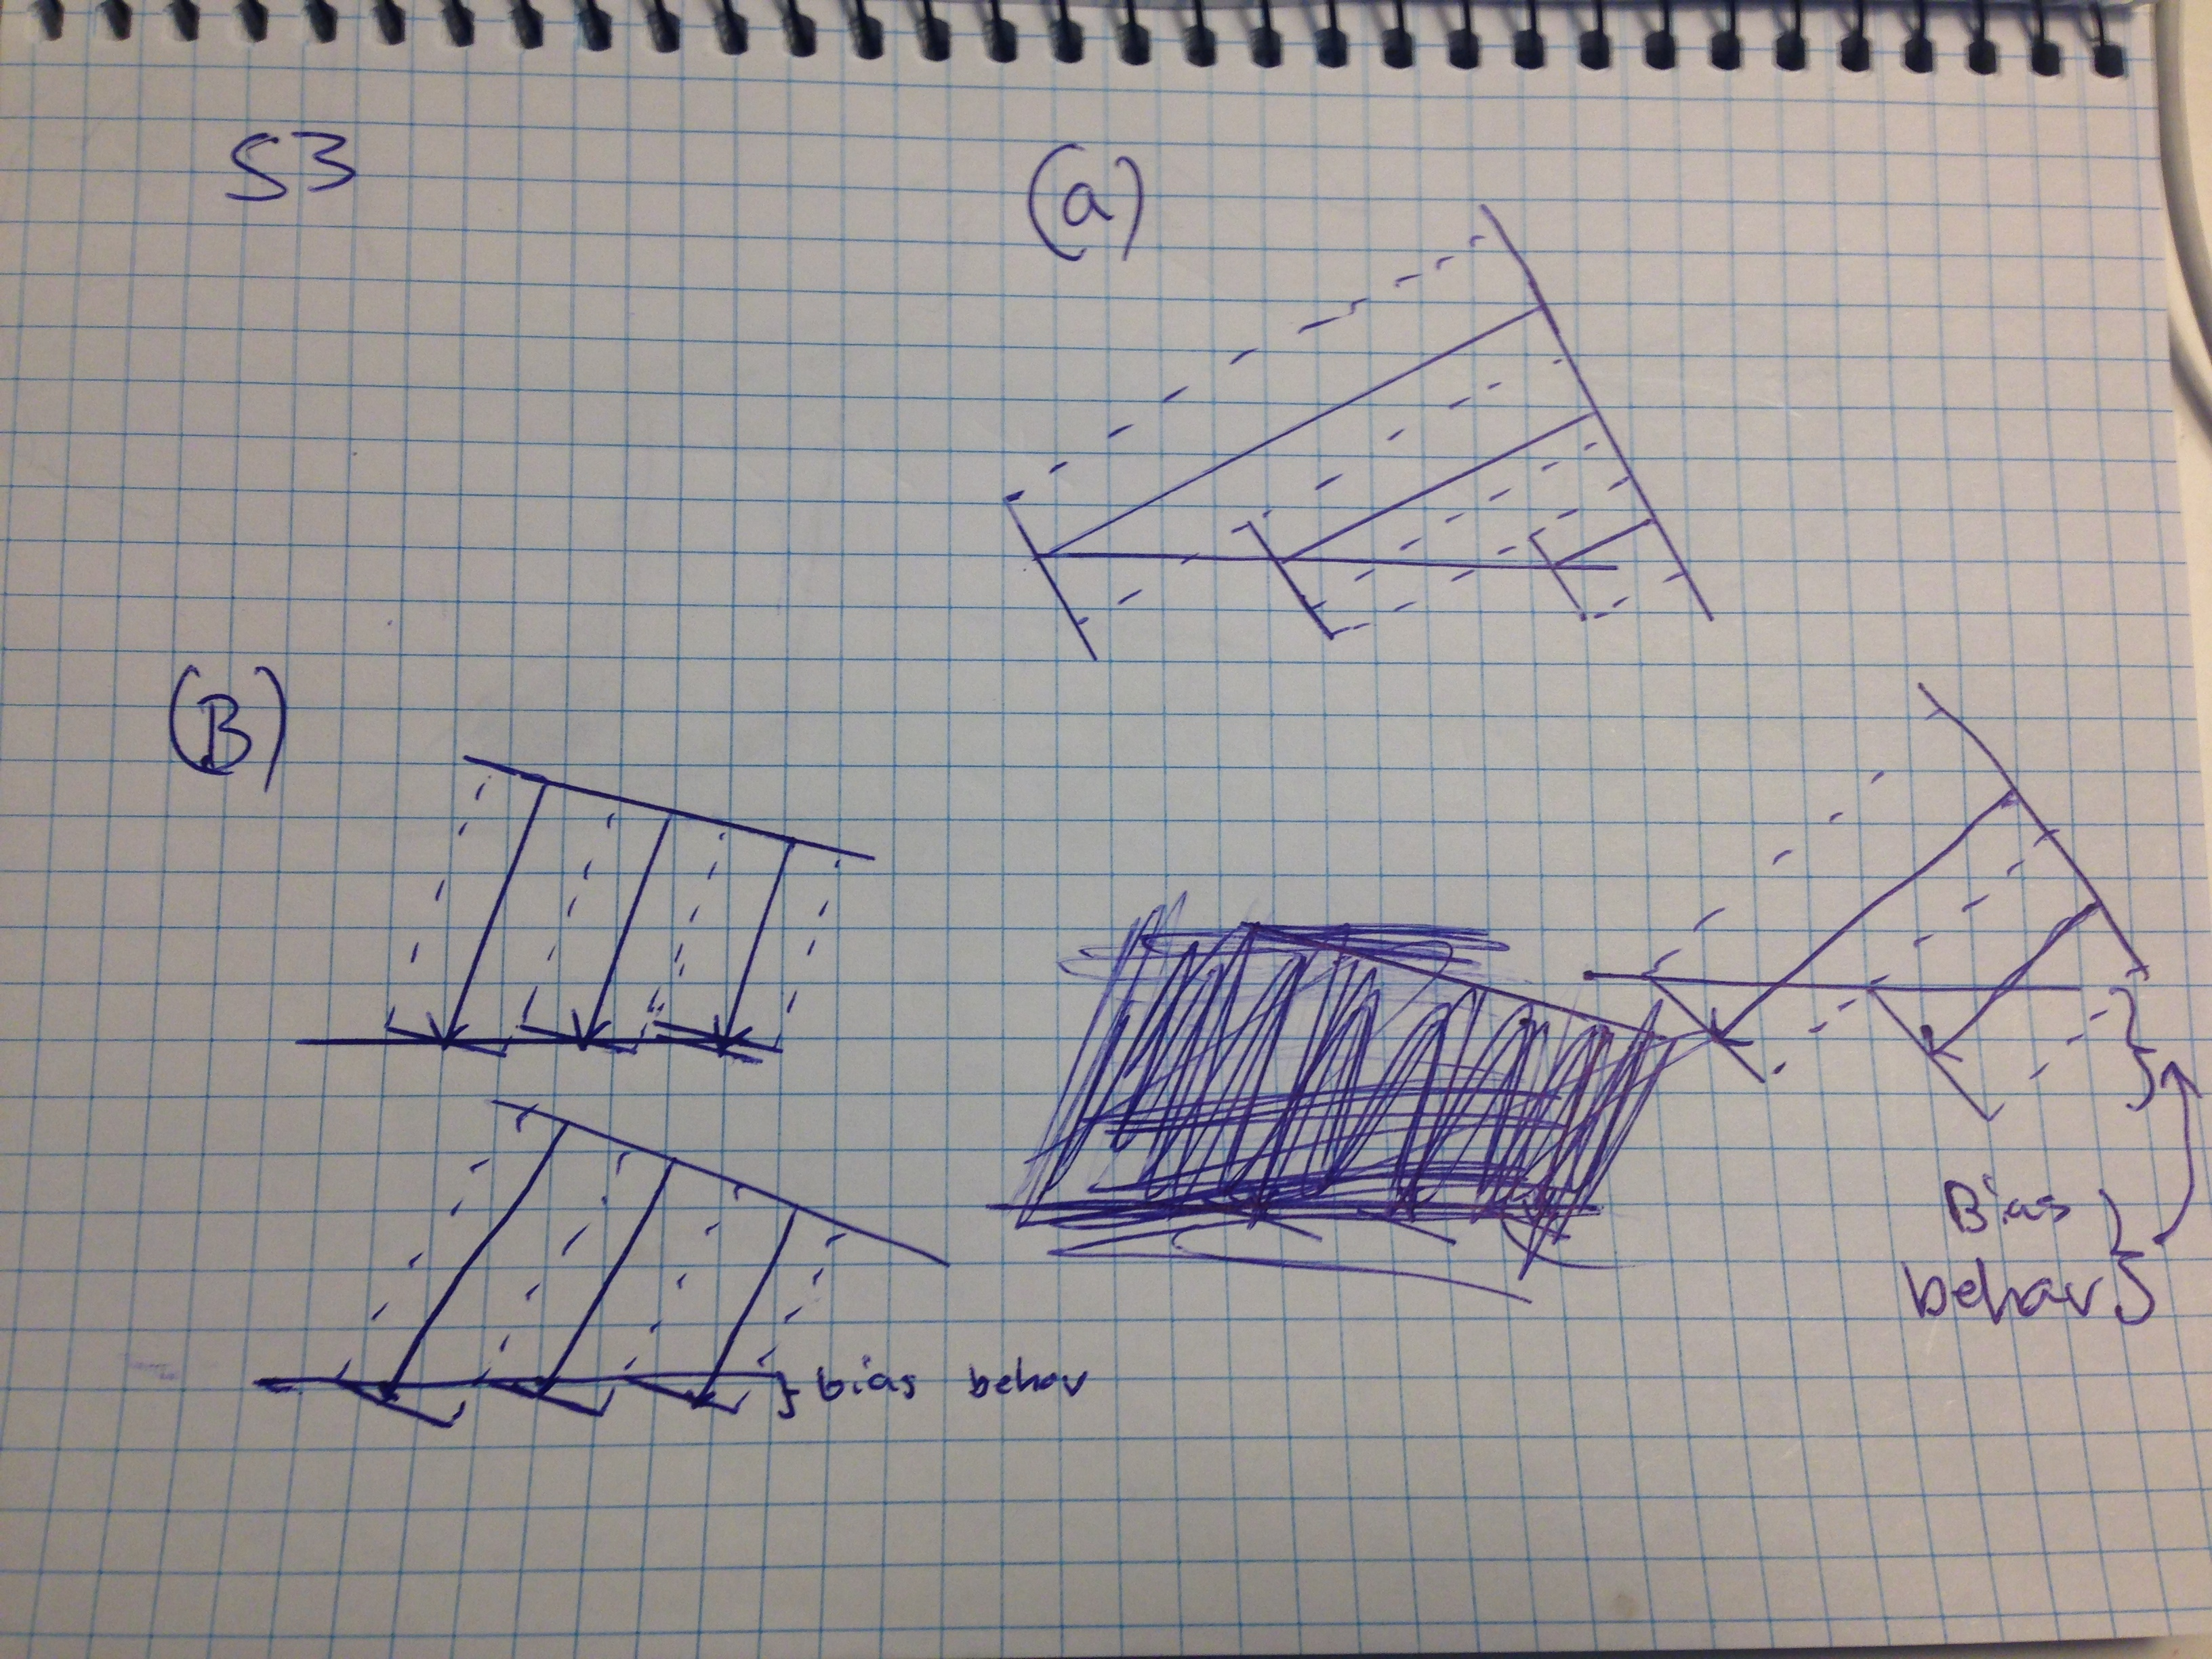
\includegraphics[width=80mm]{img/S3.jpg}
\caption{Shadow acne opstår fordi punkt samplet ikke er helt ens set fra lyset og øjet.}
\label{S3}
\end{figure}


\begin{figure}
\[ offset = m * factor + r * units \] 
\[ m = max(\frac{aZ}{ax},\frac{aZ}{aY})\]
\caption{Formlen for \textit{slop-scale bais}. \textit{r} er den mindets værdi garanteret at give en beregnelig forskel i dybde værdien. \textit{m} er den største dybde hældning  og \textit{factor} og \textit{unit} tilpasse implantationen.}
\end{figure}


Både konstant bias og slop-scale bias løser løser de to problemer der kan opstå når der foretages projektion ind i shadow mappet( geometrisk og numerisk fejl). Grunde til der ikke bare kan vælge en konstant bias værdi der altid vil være stor nok er at dette vil skabe et nyt problem kendt som Peter panning eller lys lekagese. Problemet opstår når bias værdi bliver for stor og skyggerne derved bliver løsrevet fra objekterne. Dette er et stort problem visuelt fordi objekter kommer til at se ud som om de svæver figur \ref{S4}. Derfor bruges en \textit{slop-scale bais} der sørge for der er bias nok til ikke at skabe shadow acne men ikke så meget at der opstår peter panning.

\begin{figure}[ht!]
\centering
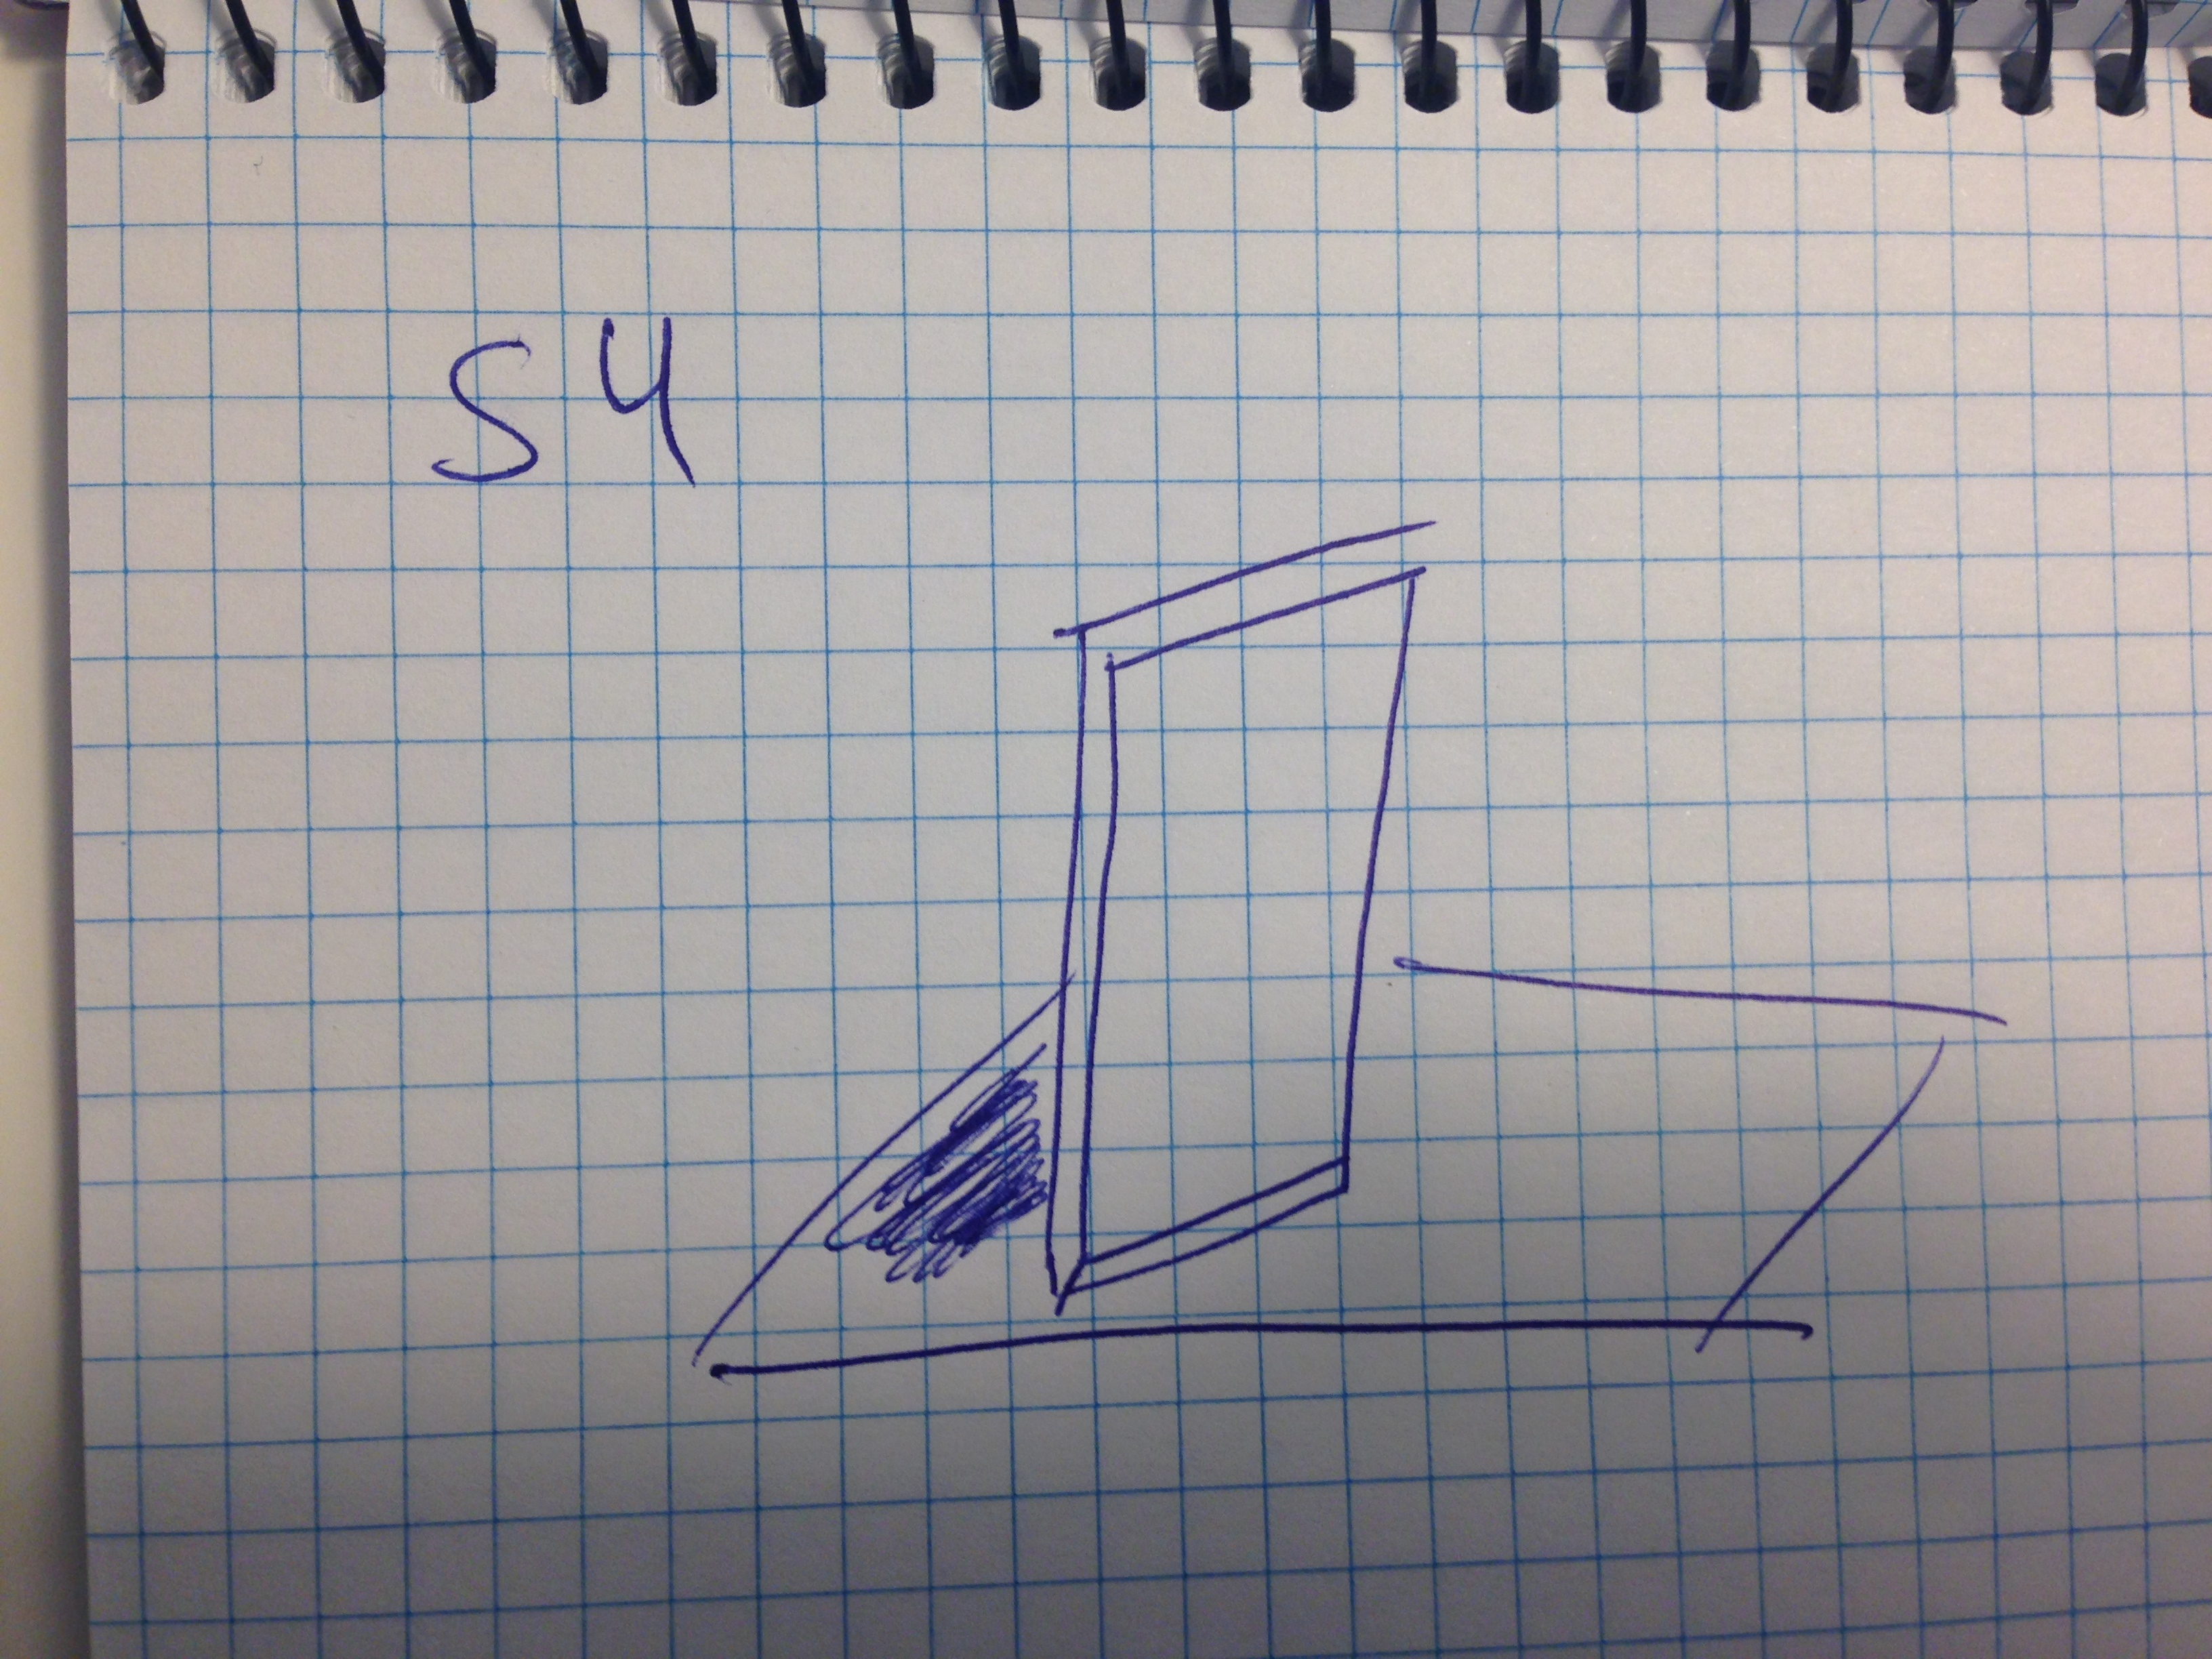
\includegraphics[width=90mm]{img/S4.jpg}
\caption{Effekt af for stor bias værdi. Dette skaber peter panning, skygger ser ud som om de er løsrevet fra figuren. Dette kan give illusion om at figure svæver selv om dette ikke er tilfældet.}
\label{S4}
\end{figure}


\newpage 

\subsection{Forbedringer/aliasing}

Shadow map  er udsat for mange aliasing problemer fordi algoritmen arbejder kun i billedopløsninger. Det kritisk at fragtmenter i kamera space bliver mappet korrekt eller så tæt som muligt på de tilsvarende pixels i shadow mappet, ellers kan skygger forekomme: kantede, jitteret eller (Selv skygge kastning er løst med bias teknikken). 

En anden grund til problemet opstår er fordi dybde bufferen ikke er lineær (er den kun for orthogonale projektion), dvs. største delen af præcisionen ligger tæt på "front clipping" planet. Dette betyder at jo længere væk objekterne er fra lyskilden jo mindre præcise vil skyggerne blive, dette bliver dog kun et problem hvis kameraet er tæt på disse objekter. 


Jeg vil her kort forklare de forskellige metode og vælge en at arbejde videre med.

\subsubsection{Percentage Closer Filtering (PCF)}

Percentage Closer Filtering(herefter referet til som PCF ) er en anti-aliasing tenik der delvist løser de problem der opstår ved oversampling. PCF teknikken blev udvilket i 1987 af Reeves, Salesin og Cook (referance). PCF kan også til dels også hjælpe på undersamplings problemet, da den udglatter skyggen og derved vil steder med undersampling ikke fremstå så kantede som uden PCF. Teknikken kan også tildels bruges til at simulere penumbra (bløde skygger) men da PCF ikke tager højde for afstande mellem lyskilden og objekt er dette ikke en penumbra algoritme. Algoritme vil dog alligevel i mange tilfælde virke overbevisende som penumbra.

PCF teknikken fungere næsten efter samme princip som ordinære texture maps i opengl, nemlig ved at sample nærliggende værdier i mappet til en middel værdi af disse. Ordinære texture maps i opengl fungere ved at først sample værdierne til en ny samplet værdi og derefter sammenligne denne. Denne tilgang vil ikke virke da der sammen lignes med dybde værdier og derfor vil give en middel dybde. I stedet byttes om på rækkefølgen så  der først sammenlignes nærliggende punkter om disse er i skygge eller ej og derefter tages et gennemsnit af værdierne og bruges som skygge værdien. figur \ref{P4} viser forskellen på de to metoder.

\begin{figure}[ht!]
\centering
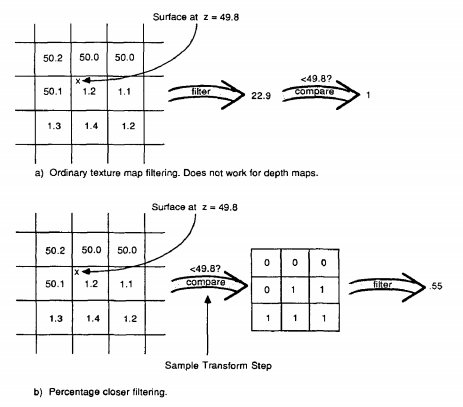
\includegraphics[width=90mm]{img/PCF1.png}
\caption{(a) ordinære texture maps i opengl. (b) PCF metoden brugt på dybde kortet.}
\label{P4}
\end{figure}


På figur \ref{P4}(b) ses hvordan PCF filteret først sammenligner dybde værdien med alle punkterne og bestemmer om punktet er i skygge eller ej, herefter tages et gennemsnit af de binære resultater hvilket bliver shadow værdien og herved får en skygger der bliver udglattet og ikke binær.


Det næste er at bestemme det område i shadow mappet der skal filteres over. Artiklen \cite{PCF} forslå to forskellig metoder at bestemme dette sampling område på.

\begin{enumerate}
\item Der anvendes en fast størrelse på omegnen der medtages af nærliggende punkter i shadow mappet
\item Nærliggende punkter på polygoniet projekteres over i shadow mappet og disse punkter bruges til at filtrese over
\end{enumerate}

Den første metode er hurtig og nem at implementere fordi der ikke skal lave nogle ekstra projektioner ind, men kun laves et antal ekstra opslag i shadow mappet følgende det størrelsen af det område der ønske. Problemet er dog at de pixel der ligger i område der filteres over ikke har nogle relation til den pixel der skal skygge farves.

Metode to kræver en del mere arbejde fordi udover punkterne skal vælges skal disse også projekteres over i shadow mappet før der kan sammenligenes og filtres over disse. Metoden burde tilgengæld i teorien give et bedre resultat da alle punkterne der filteres over ret faktisk ligger på polygonet. Denne metode har artiklen  \cite{PCF} dog ikke testet.

FORKLAR HVILKEN METODE JEG VIL BRUGE.



\newpage 
\section{Stencil Shadow Volumes}

\subsection{Teori}
Beskrivelse af Stencil shadow Volumes teknikken. heriblandt fordele og ulemper.

løser problemet med 1-1 fra cam til lys

\subsection{Depth-Pass Vs. Depth-Fail}
Sammen ligner de 2 metoder Depth-Pass og Depth-Fail for at bestemme om en vertex er i skygge eller ej.


\section{Afprøvning}
 De 2 metoder afprøves, og det vises hvordan de forskellige metoder og filtre påvirker resultaterne.	

\subsection{Køretider}
Køretiderner for de 2 metoder afprøves.

\section{Konklution}



\newpage 

\begin{thebibliography}{100} % 100 is a random guess of the total number of 
%references 
 
\addtolength{\leftmargin}{0.2in} % sets up alignment with the following line. 
\setlength{\itemindent}{-0.2in} 

\bibitem[RSC84]{PCF} 
 Rendering Antialiased Shadows with Depth Maps.
  William T. Reeves , David H. Salesin, Robert L. Cook 
  \emph{Computer Graphics, Volume 21}, 283-291, 1987.
  
  \bibitem[LW78]{SMAP} 
 CASTING CURVED SHADOWS ON CURVED SURFACES 
  Lance Williams
  \emph{Computer Graphics Lab New York Institute of Technology }, 1978.

  \bibitem[LW78]{PSMAP} 
 Perspective Shadow Maps 
  Marc Stamminger og George Drettakis.
  \emph{REVES - INRIA Sophia-Antipolis, France}, 2002.
    
  
  
\end{thebibliography} 


\end{document}